% ------------------------------------------
% MASA FORMAL TECHNICAL REPORT TEMPLATE
%  - Last updated by Theo Rulko, 12/25/2021
%  - Conforms to AE305/405 TechComm Standards
% ------------------------------------------
\documentclass{article}
\usepackage{enumerate}
\usepackage{float}
\usepackage[table,xcdraw]{xcolor}
\usepackage{array} % For fixed width in tables
\usepackage{tikz} % Image & Annotations
\usepackage{pdfpages} % Import PDF Package
\usetikzlibrary{calc} % Library to calculate X,Y AXIS
\usepackage[utf8]{inputenc}
\usepackage[english]{babel}
\usepackage{fancyhdr} %HEADER Package
\newcolumntype{L}{>{\centering\arraybackslash}m{2cm}}
% Preamble
\newcommand{\mytitle}{IHM Report : J-28012020-076}
\newcommand{\myauthors}{Varuna Marine Services BV}
\newcommand{\mydate}{May 25, 2022}

\newcommand*\annotatedFigureBoxCustom[8]{\draw[#5,thick,rounded corners] (#1) rectangle (#2);\node at (#4) [fill=#6,thick,shape=circle,draw=#7,inner sep=2pt,font=\sffamily,text=#8] {\textbf{#3}};}
%\annotatedFigureBox{bottom-left}{top-right}{label}{label-position}
\newcommand*\annotatedFigureBox[4]{\annotatedFigureBoxCustom{#1}{#2}{#3}{#4}{white}{white}{black}{black}}
\newcommand*\annotatedFigureText[4]{\node[draw=none, anchor=south west, text=#2, inner sep=0, text width=#3\linewidth,font=\sffamily] at (#1){#4};}
\newenvironment {annotatedFigure}[1]{\centering\begin{tikzpicture}
\node[anchor=south west,inner sep=0] (image) at (0,0) { #1};\begin{scope}[x={(image.south east)},y={(image.north west)}]}{\end{scope}\end{tikzpicture}}

% MASA Formal Report Template frontmatter, conforming to AE405 Standards
% Created by Theo Rulko, 25/12/2021
% Contact trulko@umich.edu with questions

% ------------------------------------------
% Import primary packages
\documentclass[english,letterpaper,11pt]{article}
\usepackage{datetime}
\usepackage[T1]{fontenc}
\usepackage{graphicx,algorithmic,algorithm}
\usepackage{color}
\usepackage{listings,url}
\usepackage{pdfpages}
\usepackage{wallpaper}
\usepackage{titlesec}
\usepackage{enumitem}
\usepackage{changepage}
\usepackage{pdfpages}
\usepackage{lscape}
\usepackage{amsmath}
\usepackage{montserrat}
\usepackage{lipsum}

% ------------------------------------------
% ToC, AIAA-style Bibliography
\usepackage[immediate]{silence}
\WarningFilter{latex}{You have requested package}
\usepackage[tocgraduated]{assets/tocstyle}
\usetocstyle{standard}
\RequirePackage[sort&compress,numbers]{natbib}
\bibliographystyle{new-aiaa}
\WarningFilter[temp]{latex}{Command}
    \usepackage{sectsty}
\DeactivateWarningFilters[temp]
\usepackage[nottoc]{tocbibind}

% ------------------------------------------
% Figures & tables
\usepackage{float}
\usepackage[small,bf]{caption}
\usepackage{tabularx}
\usepackage{multirow}
\usepackage{placeins}
\usepackage{makecell}
\usepackage[figuresleft]{rotating}

% ------------------------------------------
% Custom layout parameters
\usepackage[margin=0.75in]{geometry}
\definecolor{MASA-Blue}{RGB}{0,39,76}
\renewcommand\thesection{\arabic{section}}
\renewcommand{\bibsection}{\section{References}}
\newcommand{\boldheader}[1]{\vspace{5mm}\textbf{#1}\textbf{:}\newline}
\sectionfont{\fontsize{19}{20}\color{MASA-Blue}\fontseries{b}\fontfamily{Montserrat-TOsF}\selectfont}
\subsectionfont{\fontsize{16}{18}\color{MASA-Blue}\fontfamily{Montserrat-TOsF}\selectfont}
\subsubsectionfont{\fontseries{sb}\fontshape{n}\color{MASA-Blue}\fontfamily{Montserrat-TOsF}\selectfont}
\titlespacing{\subsection}{0pt}{100mm}{0pt}
\setlength{\parindent}{0in}
\setlength{\parskip}{1em}



% ------------------------------------------
% Letterhead
\newcommand\MASALetterhead[3]{
    \hfuzz=60pt
    \thispagestyle{empty}
    \setlength{\parskip}{0in}
    % (For full style of letterhead footer, use Footer1)
 %   \LLCornerWallPaper{1}{assets/Footer2.pdf}
    \begin{flushleft}
     %   
\includegraphics[width=4.5cm]{assets/Worm_vector.pdf}
    \end{flushleft}
    \begin{flushright}
        \begin{tabularx}{0.5\textwidth}{l @{}}#1\end{tabularx}
    \end{flushright}
    \begin{flushleft}
        \par #2 \\ \vspace{2mm} \mydate
    \end{flushleft}
    Subject: #3
    \setlength{\parskip}{1em}
}
\newcommand\signature[2]{
    \begin{minipage}{5cm}
        \noindent\vspace{4.5mm}\par
        \noindent\vspace{-1mm}\rule{#1cm}{0.5pt}\par
        \noindent#2
    \end{minipage}
}

% ------------------------------------------
% Title Page
\newcommand\makeTitlePage[1]{
    \newpage
    \ClearWallPaper
    \thispagestyle{empty}
    \setlength{\parskip}{0in}
    % (For TSM logo footer, use Footer3)
 %   \LLCornerWallPaper{1}{assets/Footer4.pdf}
    \vspace*{\fill}
    \begin{adjustwidth}{1.5cm}{1.5cm} 
    \begin{center}
      %  
\includegraphics[width=7cm]{assets/Worm_vector.pdf}\\
        \vspace{20mm}
        \fontsize{28}{30}\fontseries{b}\fontshape{n}\color{MASA-Blue}\fontfamily{Montserrat-TOsF}\selectfont{\mytitle}\\
        \vspace{15mm}
        \fontsize{14}{16}\fontseries{sb}\fontshape{n}\color{MASA-Blue}\fontfamily{Montserrat-TOsF}\selectfont{\mydate\\\vspace{7.5mm} Prepared by:}\\
        \fontsize{14}{16}\fontseries{m}\fontshape{n}\color{MASA-Blue}\fontfamily{Montserrat-TOsF}\selectfont{\myauthors}\\
        \vspace{7.5mm}
        \fontsize{14}{16}\fontseries{sb}\fontshape{n}\color{MASA-Blue}\fontfamily{Montserrat-TOsF}\selectfont{Prepared for:}\\
        \fontsize{14}{16}\fontseries{m}\fontshape{n}\color{MASA-Blue}\fontfamily{Montserrat-TOsF}\selectfont{#1}
        \vspace{50mm}
    \end{center}
    \end{adjustwidth}
    \vspace*{\fill}
    \setlength{\parskip}{1em}
}

% ------------------------------------------
% Cover Page
\newcommand\makeCoverPage{
    \newpage
    \ClearWallPaper
    \thispagestyle{empty}
    \setlength{\parskip}{0in}
    % (For TSM logo footer, use Footer3)
   % \LLCornerWallPaper{1}{assets/Footer4.pdf}
    \vspace*{\fill}
    \begin{adjustwidth}{1.5cm}{1.5cm} 
    \begin{center}
     %   
\includegraphics[width=9cm]{assets/Worm_vector.pdf}\\
        \vspace{25mm}
        \fontsize{33}{35}\fontseries{b}\fontshape{n}\color{MASA-Blue}\fontfamily{Montserrat-TOsF}\selectfont{\mytitle}
        \vspace{45mm}
    \end{center}
    \end{adjustwidth}
    \vspace*{\fill}
    \setlength{\parskip}{1em}
}

% ------------------------------------------
% Acknowledgements
\newcommand\MASAacknowledgements[1]{
    \newpage
    \topskip0pt
    \addcontentsline{toc}{section}{Acknowledgements}
    \vspace*{\fill}
    \begin{adjustwidth}{1.5cm}{1.5cm} 
    \begin{center}
    \textbf{\Large\color{MASA-Blue}\fontfamily{Montserrat-TOsF}\selectfont Acknowledgements}\\
    \vspace{5mm}
    \end{center}
    #1
    \end{adjustwidth}
    \vspace*{\fill}
}

% ------------------------------------------
% Format for matlab code listing
\usepackage{listings}
\definecolor{commentgreen}{RGB}{14,120,0}
\lstset{
    numbers=left, 
    basicstyle=\scriptsize, 
    commentstyle=\color{commentgreen},
    keywordstyle=\bf\color{blue},
    language=matlab, 
    frame=leftline,
    rulesepcolor=\color{black},
    flexiblecolumns=true,
    extendedchars=false,
    keepspaces=true
}

% ------------------------------------------
% Custom Math Shorthand (Credit: kfid@umich.edu)
\newcommand{\pp}[2]{\dfrac{\partial #1}{\partial #2}}
\newcommand{\ppt}[2]{\dfrac{\partial^2 #1}{\partial #2^2}}
\newcommand{\DD}[2]{\dfrac{D #1}{D #2}}
\newcommand{\dd}[2]{\dfrac{d #1}{d #2}}
\newcommand{\mbb}[1]{\mathbb{#1}}
\newcommand{\mbf}[1]{\mathbf{#1}}
\newcommand{\mrm}[1]{\mathrm{#1}}
\newcommand{\mcal}[1]{\mathcal{#1}}
\newcommand{\BigO}{\mathcal{O}}
\newcommand{\norm}[2]{\left\lVert{#1}\right\lVert_{#2}}
\newcommand{\sbf}[1]{\boldsymbol{#1}}
\def\etal{{\it et al~}}
\newcommand{\be}{\begin{eqnarray}}
\newcommand{\ee}{\end{eqnarray}}
\newcommand{\ben}{\begin{eqnarray*}}
\newcommand{\een}{\end{eqnarray*}}
\newcommand{\dx}{d\mbf{x}}
\newcommand{\Dt}{\Delta t}
\newcommand{\ih}{\hat{i}}
\newcommand{\jh}{\hat{j}}
\newcommand{\kh}{\hat{k}}
\newcommand{\xh}{\hat{x}}
\newcommand{\yh}{\hat{y}}
\newcommand{\zh}{\hat{z}}
\newcommand{\Uinf}{U_{\infty}}
\newcommand{\Vinf}{V_{\infty}}
\newcommand{\Minf}{M_{\infty}}
\newcommand{\bVinf}{\mbf{V}_{\infty}}
\newcommand{\scriptth}{\scriptsize \textnormal{th}}
\newcommand{\half}{\frac{1}{2}}
\newcommand{\CFL}{{\mbox{CFL}}}
\newcommand{\tn}[1]{\textnormal{#1}}
\newcommand{\mbfh}[1]{\widehat{\mathbf{#1}}}
\newcommand{\m}{\textrm{m}}
\newcommand{\s}{\textrm{s}}
\newcommand{\kg}{\textrm{kg}}
\newcommand{\km}{\textrm{km}}
\newcommand{\N}{\textrm{N}}
\newcommand{\Pa}{\textrm{Pa}}
\newcommand{\K}{\textrm{K}}
\newcommand{\C}{\textrm{C}}
\newcommand{\mbfv}[1]{\vec{\mathbf{#1}}}
\newcommand{\comment}[1]{}
\pagestyle{fancy}
\fancyhf{}
\fancyhead[LE,RO]{IMO: 9485899}
\fancyhead[RE,LO]{Varuna Marine Services}
% \fancyhead[CE,LO]{Project Number}
\fancyfoot[CE,CO]{Varuna Marine Services, Middelburgsestraat 1C, 2587 CS, The Hague, The Netherlands, varunamarine.eu}
\fancyfoot[LE,RO]{\thepage}
\begin{document}

% ------------------------------------------
% TITLE PAGE, COVER PAGE, ACKNOWLEDGEMENTS, TABLES
% ------------------------------------------
% Cover and title pages
\makeCoverPage
\makeTitlePage{AS Elenia IMO No.: 9485899} % (Prepared for)

% Acknowledgements page
%\MASAacknowledgements{
%    \lipsum[3]\vspace{5mm}\\
%    This project was supported by funding provided by MASA at the University of Michigan, Ann %Arbor.
%}

\ClearWallPaper % (Removes letter/cover footer graphic from subsequent pages)
\pagenumbering{roman}

% Tables of contents, figures, tables
\begin{center}
\renewcommand{\arraystretch}{1.6}
% Please add the following required packages to your document preamble:
% \usepackage[table,xcdraw]{xcolor}
% If you use beamer only pass "xcolor=table" option, i.e. \documentclass[xcolor=table]{beamer}
\begin{table}[]
\begin{tabular}{|l|l|}
\hline
\textbf{IMO Number}               & 9485899                                                                                                                                                                                                                                                        \\ \hline
\textbf{Name of Ship}             & AS Elenia                                                                                                                                                                                                                                                      \\ \hline
\textbf{Type}                     & Bulk Carrier                                                                                                                                                                                                                                                   \\ \hline
\textbf{Flag}                     & Liberia                                                                                                                                                                                                                                                        \\ \hline
\textbf{Port of Registry}         & Manrovia                                                                                                                                                                                                                                                       \\ \hline
\textbf{Class Society}            & DNV GL                                                                                                                                                                                                                                                         \\ \hline
\textbf{Gross tonnage (GT)}       & 23443 T                                                                                                                                                                                                                                                        \\ \hline
\textbf{Dimensions (L x B x D)}   & 180 m x 30 m x 14.70 m                                                                                                                                                                                                                                         \\ \hline
\textbf{Date of building}         & 2011                                                                                                                                                                                                                                                           \\ \hline
\textbf{Date of delivery}         & 2011                                                                                                                                                                                                                                                           \\ \hline
\textbf{Ship builder}             & \begin{tabular}[c]{@{}l@{}}SPP Shipbuilding Co., Ltd\\ Sacheon-si, Gyeongsangnam-do 664-942, KR\end{tabular}                                                                                                                                                   \\ \hline
\textbf{Shipowner}                & \begin{tabular}[c]{@{}l@{}}Nordic Handysize III AS\\ Munkedamsveien 62C, 0270 Oslo\\ Postal address:\\ c / o Clarksons Platou Project F AS Munkedamsveien 62C, 0270\\ Oslo\end{tabular}                                                                        \\ \hline
\textbf{Ship manager}             & \begin{tabular}[c]{@{}l@{}}Blue squared AG\\ Taubenstrasse 32\\ CH-3011 Bern\\ Switzerland\end{tabular}                                                                                                                                                        \\ \hline
\textbf{Date of ship inspection}  & 2022-09-24                                                                                                                                                                                                                                                     \\ \hline
\textbf{Place of ship inspection} & \begin{tabular}[c]{@{}l@{}}Zhenjiang\\ China\end{tabular}                                                                                                                                                                                                      \\ \hline
\textbf{Surveyors}                & Gao Qi (Hazmat Expert, Varuna Marine Services)                                                                                                                                                                                                                 \\ \hline
\textbf{Laboratories}             & \begin{tabular}[c]{@{}l@{}}Suzhou FALAB Test Technology Co.,LTD\\ Suzhou FALAB Test Technology Co.,LTD\\ Shanghai Office: Room 201, Building A8, No 1600 North Guo\\ Quan Road, Yangpu Region,Shanghai City, P.R. China\\ Web:http://www.falab.cn\end{tabular} \\ \hline
\end{tabular}
\end{table}
\end{center}
\newpage
\section{Quality}
We are committed to providing customers with service of the highest possible level of quality. In order to achieve this, we are continually improving processes, products and services, meeting and exceeding customer satisfaction at all times. It is compulsory that all staff recognize and accept our philosophy of quality service delivery, accepting accountability for their own output.
\section{Disclaimer}
Varuna Marine Services does not warrant or assume any kind of liability for the up-to-date nature, accuracy,
completeness or quality of the HazMat weight calculation provided. Liability claims against any member of
Varuna Marine Services in relation to any loss or damage arising out of or in connection with the use or nonuse of HazMat weight calculation provided, including the use of incorrect or incomplete HazMat weight
calculation data, are excluded to the fullest extent permissible by law. All weight calculation data may be
subject to alteration and are non-binding. Each Varuna Marine Services member expressly reserves the
right without notice to change, supplement or delete parts of the HazMat weight calculation data or to stop
the publication and usage temporarily or definitively.
\section{Copyright © 2019 All rights reserved}
No part of these pages, either text or image may be reproduced, and / or made public in any form or by any
means, electronic, mechanical or otherwise, without prior written permission, by Varuna Marine Services,
Middelburgsestraat 1C, 2587 CS, The Hague, The Netherlands.

\newpage
\tableofcontents
\newpage
\listoffigures
\newpage
\listoftables

% ------------------------------------------
% REPORT BODY
% ------------------------------------------
\newpage \pagenumbering{arabic} \setcounter{page}{1}

\section{Introduction}
This “Inventory of hazardous materials” (hereinafter referred to as the "IHM" or
“the inventory”) was prepared in accordance with Resolution MEPC.269(68)
adopted on 15 MAY 2015 (2015 Guidelines for the development of the Inventory
of hazardous materials).
2015 Guidelines provide recommendations for developing the Inventory of
Hazardous Materials to assist compliance with regulation 5 (Inventory of
Hazardous Materials) of the “Hong Kong International Convention for the Safe
and Environmentally Sound Recycling of Ships, 2009” (hereinafter referred to as
"the Convention") and article 5 of the “Regulation (EU) No.1257/2013 of the
European Parliament and of the Council of 20 November 2013 on ship recycling”.

% -----------------------------------------
\newpage
\section{Methodology and Scope}

\subsection{Objectives}
The objectives of the Inventory are to provide shipspecific information on the
actual Hazardous Materials present on board, in order to protect health and
safety and to prevent environmental pollution at Ship Recycling Facilities. This
information will be used by the Ship Recycling Facilities in order to decide how to
manage the types and amounts of materials identified in the Inventory of
Hazardous Materials (regulation 9 of the Ship Recycling Convention).

\subsection{Process for checking of materials}
In order to develop part I of the Inventory for existing ships, the following
procedure has been applied.
\subsection{Materials to be listed in part I of the Inventory}
\begin{enumerate}
\item Table A comprises the materials listed in appendix 1 of the Convention;
Asbestos
\subitem Asbestos
\subitem Polychlorinated biphenyls (PCBs)
\subitem Ozone Depleting Substances (ODS)
\subitem Anti-fouling systems containing organotin compounds as a biocide (TBT)
\item Table B comprises the materials listed in appendix 2 of the Convention; (as
far as practicable)
\subitem Cadmium and Cadmium Compounds
\subitem Hexavalent Chromium Compounds
\subitem Mercury and Mercury Compounds
\subitem Lead and Lead Compounds
\subitem Polybrominated Biphenyl (PBBs)
\subitem Polybrominated Diphenyl Ethers (PBDE)
\subitem Polychlorinated Naphthalenes
\subitem Radioactive Substances
\subitem Certain Short Chain Chlorinated Paraffins
\item The two additional hazardous materials as per EU SRR, if applicable
\subitem Perfluorooctane sulfonic acid (PFOS)
\subitem Brominated Flame Retardant (HBCDD)

\end{enumerate}

\section{Collection of necessary information}

\subsection{Sighting of available documents}

The information collected from following documents was assessed.
And the results of the assessment was reflected in the visual/sampling check
plan.

\begin{enumerate}

\item Ship's specification
\item General Arrangement
\item Machinery Arrangement
\item Spare Parts and Tools List
\item Piping Arrangement
\item Accommodation Plan
\item Fire Control Plan
\item Fire Protection Plan
\item Insulation Plan (Hull and Machinery)
\item International Anti-Fouling System Certificate
\item International Air Pollution Prevention Certificate
\item Related manuals and drawings
\item Information from other inventories and/or sister or similar ships,
machinery, equipment, materials and coatings, if applicable
\item Results of previous visual/sampling checks and other analysis, if applicable

\end{enumerate}
\subsection{Indicative lists}
It is impossible to check all equipment, systems, and/or areas on board the ship
to determine the presence or absence of hazardous materials since the total
number of parts on board may exceed several thousands. In order to take a
practical approach, indicative lists have been used to identify the equipment,
system, and/or area on board that is presumed to contain hazardous
substances.
A typical example of an indicative list is shown below.

\subsubsection{Table A, Asbestos}

% Please add the following required packages to your document preamble:
% \usepackage{multirow}
\begin{center}
\renewcommand{\arraystretch}{1.4}
\begin{table}[H]
\begin{tabular}{|l|l|}
\hline
\textbf{Structure and/or equipment} & \textbf{Component}                                                                                                                       \\ \hline
\multirow{5}{*}{Propeller shafting} & Packing with low pressure hydraulic piping flange                                                                                        \\ \cline{2-2} 
                                    & Packing with casing                                                                                                                      \\ \cline{2-2} 
                                    & Clutch                                                                                                                                   \\ \cline{2-2} 
                                    & Brake lining                                                                                                                             \\ \cline{2-2} 
                                    & Synthetic stern tubes                                                                                                                    \\ \hline
\multirow{4}{*}{Diesel Engine}      & Packing with piping flange                                                                                                               \\ \cline{2-2} 
                                    & Lagging material for fuel pipe                                                                                                           \\ \cline{2-2} 
                                    & Lagging material for exhaust pipe                                                                                                        \\ \cline{2-2} 
                                    & Lagging material for turbo charger                                                                                                       \\ \hline
\multirow{3}{*}{Turbo Engine}       & Lagging material for casing                                                                                                              \\ \cline{2-2} 
                                    & \begin{tabular}[c]{@{}l@{}}Packing with flange of piping and valve for steam line,\\ exhaust line and drain line\end{tabular}            \\ \cline{2-2} 
                                    & \begin{tabular}[c]{@{}l@{}}Lagging material for piping and valve of steam line,\\ exhaust line and drain line\end{tabular}               \\ \hline
\multirow{8}{*}{Boiler}             & Insulation in combustion chamber                                                                                                         \\ \cline{2-2} 
                                    & Packing for casing door                                                                                                                  \\ \cline{2-2} 
                                    & Lagging material for exhaust pipe                                                                                                        \\ \cline{2-2} 
                                    & Gasket for manhole                                                                                                                       \\ \cline{2-2} 
                                    & Gasket for hand hole                                                                                                                     \\ \cline{2-2} 
                                    & Gas shield packing for soot blower and other hole                                                                                        \\ \cline{2-2} 
                                    & \begin{tabular}[c]{@{}l@{}}Packing with flange of piping and valve for steam line,\\ exhaust line, fuel line and drain line\end{tabular} \\ \cline{2-2} 
                                    & \begin{tabular}[c]{@{}l@{}}Lagging material for piping and valve of steam line,\\ exhaust line, fuel line and drain line\end{tabular}    \\ \hline
\end{tabular}
\end{table}
\end{center}

\subsubsection{Table A, Polychlorinated Biphenyls (PCB)}
\renewcommand{\arraystretch}{1.4}
\begin{center}
\begin{table}[H]
\begin{tabular}{|l|l|}
\hline
\textbf{Equipment} & \textbf{Component of equipment} \\ \hline
Transformer        & Insulating oil                  \\ \hline
Condenser          & Insulating oil                  \\ \hline
Fuel heater        & Heating medium                  \\ \hline
Electrical cable   & Covering, insulating tape       \\ \hline
Lubrication oil    &                                 \\ \hline
Heat oil           &                                 \\ \hline
\end{tabular}
\end{table}
\end{center}

\subsubsection{Table A, Ozone Depleting Substances (ODS)}
\renewcommand{\arraystretch}{1.4}
\begin{center}
\begin{table}[H]
\begin{tabular}{|l|l|}
\hline
\textbf{Materials} & \textbf{Component of equipment} \\ \hline
CFCs (R11, R12)        & Refrigerant for refrigerators              \\ \hline
CFCs          & Urethane formed material                  \\ \hline
Halons      & Extinguishing agent                 \\ \hline
Other fully halogenated CFCs   & The possibility of usage in ship is low.       \\ \hline
Carbon tetrachloride    &        The possibility of usage in ship is low.The possibility of usage in ship is low.                         \\ \hline
1,1,1-Trichloroethane (Methyl
chloroform)          &              The possibility of usage in ship is low.                   \\ \hline
\end{tabular}
\end{table}
\end{center}

\subsubsection{Table A, Organotin compounds}
Organotin compounds include tributyl tins (TBT), triphenyl tins (TPT) and tributyl
tin oxide (TBTO). Organotin compounds have been used as anti-fouling paint on
ships' bottoms.

\subsubsection{EU - SRR, Perfluorooctane sulfonic acid (PFOS)}
In the marine industry, it can be found in fire-fighting foams on vessels carrying
inflammable fluids and those with helicopter decks, rubber and plastic materials
(i.e.: cable sheaths, PVC flooring, gaskets and seals) and coatings (i.e.: paint). An
indicative list of materials and components that may contain PFOS is the
following:
\begin{itemize}
    \item FFFP (Film-forming Fluor-protein foams): used for aviation and shallow spill
fires
\item AR-AFFF (Alcohol-resistant aqueous film-forming foams): multi-purpose
foams
\item AR-FFFP (Alcohol-resistant film-forming flour-protein foams): multipurpose
foams developed in the 1970s
\item Hydraulic fluids
\item Cable sheath
\item Coating
\item Adhesives
\end{itemize}

\subsection{Exclusions}
Materials listed in Table B of that are inherent in solid metals or metal alloys,
such as steels, aluminium, brasses, bronzes, plating and solders, provided they
are used in general construction, such as hull, superstructure, pipes or housings
for equipment and machinery, are not required to be listed in the Inventory.
Although electrical and electronic equipment is required to be listed in the
Inventory, the amount of hazardous materials potentially contained in printed
wiring boards (printed circuit boards) installed in the equipment does not need
to be reported in the Inventory. \\ \\
In case of the loosely fitted equipment present on board the ship, such as fire
extinguishers, distress flares, and lifebuoys is no need to list in part I of the
Inventory. Such equipment which remains on board when the ship is recycled
should be listed in part III (Stores).\\ \\
Furthermore, Table C and table D materials corresponding to part II and/or III
are excluded from the scope investigation. \\ \\
If the equipment, system and/or area of the ship are not accessible for a visual
check or sampling check, they will be classified as “potentially containing
hazardous material”(PCHM). Any equipment, system and/or area classed as
“potentially containing hazardous material” may be investigated or subjected to
a sampling check at the request of the shipowner during a later survey (e.g.
during repair, refit, or conversion).

\section{Assessment of collected information}
The information collected in Sec.3.1 above was assessed. Based on collected
information, all equipment, systems, and/or areas on board assumed to contain
hazardous materials listed in table A and B of the Res.MEPC.269(68) was
reflected in the visual/sampling check plan.

\section{Preparation of Visual Sampling Check Plan (VSCP)}
To specify the materials listed in appendix 1 of the Res.MEPC.269(68), a visual
/sampling check plan was prepared taking into account the collated information
and appropriate expertise. \\ \\
Each item classified as "Contained" or "Not contained" in the checklist was
checked visually. For each item categorized as “Unknown”, are checked visually
and/or checked by sampling. \\ \\
However, any item categorized as “Unknown” may be classed as “potentially
containing hazardous material” provided comprehensive justification is given, or
if it can be assumed that there will be little or no effect on disassembly as a unit
and later ship recycling and disposal operations. \\ \\
Furthermore, items listed in the visual/sampling check was arranged in
sequence so that the onboard check is conducted in a structured manner (e.g.
from a lower level to an upper level and from a fore part to an aft part). 

\section{Onboard visual/sampling check}

\subsection{General description}

The onboard visual/sampling check was carried out in accordance with the visual
/sampling check plan and the check points were marked in the ship’s plan or
recorded with photographs. The results of visual/sampling checks were
recorded in the checklist. Any equipment, systems and/or areas of the ship that
cannot be accessed for checks were classified as "potentially containing
hazardous material". \\ \\
Each person taking samples during onboard visual/sampling check wore the
appropriate safety equipment relevant to the suspected type of hazardous
materials encountered. Appropriate safety precautions such as posting of signs
or other verbal or written notice have been put in place for crewmembers and
other person on board, to minimize the potential exposure to hazardous
materials.

\subsection{Methodology using CyberSmart}
Cyber Smart has been used to prepare and guide the onboard visual/sampling
check. Afterwards the collected data was reviewed and enhanced by using the
software.

\subsubsection{Preparation}

The General Arrangement Plan(s) were imported into CyberSmart and used to
define logical decks/deckplans used in the software. These deckplans were
named and ordered in a way to help the onboard sampling procedure. \\ \\
VSCP entries were created with the software using the prepared deckplans to
describe the objects and their locations to check by selecting appropriate
deckplans and picking exact locations on them if applicable \\ \\

\subsubsection{Sample Identification (numbering}
Each sample and visual check got assigned an unique identifier by the software.
Physical label tags were attached to the sample bags each containing a unique
number in a custom numbering system. Additionally these label tags might
contain NFC tags and/or a visual encodings (i.e. Barcode, QR Code) of the
printed number to help tool assisted identification with CyberSmart App or
compatible NFC readers or Barcode scanners.

\subsubsection{Data recording with CyberSmart App}
Checks performed with the Cyber Smart App got recorded by following this
automatically guided process:

\begin{enumerate}
    \item a relevant VSCP entry got chosen from the deckplan or from a list as
starting point (optional)
\item the check's location was specified on the deckplan as exact as possible
\item the check's data (location, object description, HazMat details, ...) was
specified (or reviewed and refined if based on a VSCP entry)
\item the check was optionally paired with a tag, e.g. NFC or QR Code on the
associated sample bag
\item at least one photo got taken of the sample an/or sampling location
\end{enumerate}
A status about the completeness of the check recording based on this process
was displayed to avoid forgetting to record information.

\subsubsection{Compilation into Report}
The recored check data got reviewed after the onboard survey to avoid potential
data errors. All performed checks are listed in this report together with their
associated data and photos.

\subsection{Samples and analysis}
The analysis of samples has been carried out by the suitably accredited
laboratory, working to international standards (e.g. ISO 17025) or an equivalent.
And also specific testing was conducted in accordance with IMO guidelines or
any equivalent method which can demonstrate equivalent standards. And the
results of the analysis have been documented in a written report that can be
relied upon by all parties.

\section{Maintaining part I of the Inventory during operation}
Part I of the Inventory should be appropriately maintained and updated,
especially after any repair or conversion or sale of a ship. \\ \\

If any machinery or equipment is added to, removed or replaced or the hull
coating is renewed, part I of the Inventory should be updated according to the
requirements for new ships as stipulated in paragraphs 4.1.2 to 4.1.4 of the Res.
MEPC.269(68). \\ \\
Updating is not required if identical parts or coatings are installed or applied. \\ \\
Part I of the Inventory should belong to the ship and the continuity and
conformity of the information it contains should be confirmed, especially if the
flag, owner or operator of the ship changes.

\section{Abbreviations and Colour Conventions}

Names, abbreviation and colour conventions used in the following chapters.



\renewcommand{\arraystretch}{1.4}
\begin{center}
\begin{table}[H]
\begin{tabular}{|ll|l|ll|}
\hline
\multicolumn{2}{|l|}{\textbf{Hazardous Material}}          & \textbf{Abbreviation} & \multicolumn{2}{l|}{\textbf{Colour}}                   \\ \hline
\multicolumn{1}{|l|}{A-1} & Asbestos                       & Asb                   & \multicolumn{1}{l|}{\cellcolor[HTML]{3531FF}} & Blue   \\ \hline
\multicolumn{1}{|l|}{A-2} & Polychlorinated Biphenyl (PCB) & PCB                   & \multicolumn{1}{l|}{\cellcolor[HTML]{6200C9}} & Purple \\ \hline
\multicolumn{1}{|l|}{A-3}    &  Ozone Depleting Substances (ODS)                               &         ODS   &           \multicolumn{1}{l|}{\cellcolor[HTML]{EBF909}} & Yellow      \\ \hline
\multicolumn{1}{|l|}{A-5 }    &  Perfluorooctane Sulfonic Acid (PFOS)                               &         PFOS    &           \multicolumn{1}{l|}{\cellcolor[HTML]{F9BA09}} & Orange      \\ \hline
\multicolumn{1}{|l|}{B-1 }    &  Cadmium (and compounds)                               &         Cd    &           \multicolumn{1}{l|}{\cellcolor[HTML]{900C3F}} & Maroon      \\ \hline
\multicolumn{1}{|l|}{B-2 }    &  Chromium (and compounds)                                &         Cr    &           \multicolumn{1}{l|}{\cellcolor[HTML]{9F4C26}} & Brown      \\ \hline
\multicolumn{1}{|l|}{B-3 }    &  Lead (and compounds)                                &         Pb    &           \multicolumn{1}{l|}{\cellcolor[HTML]{908D8C}} & Grey      \\ \hline
\multicolumn{1}{|l|}{B-4 }    &  Mercury (and compounds)                                &         Hg    &           \multicolumn{1}{l|}{\cellcolor[HTML]{A778E9}} & Lavender      \\ \hline
\multicolumn{1}{|l|}{B-5}    &  Polybrominated Biphenyl (PBB)                                &         PBB    &           \multicolumn{1}{l|}{\cellcolor[HTML]{18B0F5}} & Cyan      \\ \hline
\multicolumn{1}{|l|}{B-6 }    &  Polybrominated Diphenyl Ethers (PBDE)                                 &         PBDE    &           \multicolumn{1}{l|}{\cellcolor[HTML]{F518C7}} & Magenta      \\ \hline
\multicolumn{1}{|l|}{B-7}    &  Polychlorinated Naphthalenes (Cl3) )                                 &         PCN    &           \multicolumn{1}{l|}{\cellcolor[HTML]{DEF518}} & Lime      \\ \hline
\multicolumn{1}{|l|}{B-8 }    &  Radioactive Material                                 &         Radio    &           \multicolumn{1}{l|}{\cellcolor[HTML]{6DF518}} & Green      \\ \hline
\multicolumn{1}{|l|}{B-9}    &  Certain Short Chain Chlorinated Paraffins                                 &         SCCP    &           \multicolumn{1}{l|}{\cellcolor[HTML]{F518D4}} & Pink      \\ \hline
\multicolumn{1}{|l|}{B-10}    &  Hexabromocyclododecane (HBCDD)                                 &         HBCDD    &           \multicolumn{1}{l|}{\cellcolor[HTML]{0B421B}} & Teal      \\ \hline
\end{tabular}
\end{table}
\end{center}

\renewcommand{\arraystretch}{1.4}
\begin{center}
\begin{table}[H]
\begin{tabular}{|l|l|l|}
\hline
\rowcolor[HTML]{C0C0C0} 
\textbf{Document Analysis Result} & \textbf{Abbreviation} & \textbf{Description}                                                                                                                                                     \\ \hline
Unknown                           & Unknown               & \begin{tabular}[c]{@{}l@{}}The document analysis for subjected object did not\\ lead to any result. A check is required for further result\\ determination.\end{tabular} \\ \hline
Not contained                     & No                    & \begin{tabular}[c]{@{}l@{}}Analyzed object has been found to not contain\\ hazardous material\end{tabular}                                                               \\ \hline
PCHM                              & PCHM                  & \begin{tabular}[c]{@{}l@{}}Documents subjecting analyzed object indicate a\\ potential containment of hazardous material.\end{tabular}                                   \\ \hline
Contained                         & Yes                   & \begin{tabular}[c]{@{}l@{}}Documents subjecting analyzed object indicate\\ containment of hazardous material.\end{tabular}                                               \\ \hline
\end{tabular}
\end{table}
\end{center}

\renewcommand{\arraystretch}{1.4}
\begin{center}
\begin{table}[H]
\begin{tabular}{|l|l|l|}
\hline
\rowcolor[HTML]{C0C0C0} 
\textbf{Check Result } & \textbf{Abbreviation} & \textbf{Description}                                                                                                                                                     \\ \hline
Not contained                           & No               & \begin{tabular}[c]{@{}l@{}}Checked object has been found to not contain
hazardous material.\end{tabular} \\ \hline
Below threshold                    & BT                    & \begin{tabular}[c]{@{}l@{}}Checked object contains hazardous material in
quantity below threshold\end{tabular}                                                               \\ \hline
PCHM                              & PCHM                  & \begin{tabular}[c]{@{}l@{}}Checked object has been found to potentially contain
hazardous material.\end{tabular}                                   \\ \hline
Contained                         & Yes                   & \begin{tabular}[c]{@{}l@{}}Checked object contains hazardous material.\end{tabular}                                               \\ \hline
\end{tabular}
\end{table}
\end{center}

\section{Visual Sampling Check Plan (VSCP)}

This chapter contains all checkpoints as prepared in the VSCP. The entries are
grouped by their associated decks and their locations marked on the
corresponding deck plans if applicable.

\subsection{Planned checkpoints: NAV. BRI. DECK}
\renewcommand{\arraystretch}{1.4}
\begin{center}
\begin{table}[H]
\begin{tabular}{|l|l|l|l|l|l|}
\hline
\textbf{No} & \textbf{\begin{tabular}[c]{@{}l@{}}Location, Compartment,\\ System\end{tabular}} & \textbf{\begin{tabular}[c]{@{}l@{}}Function, Equipment,\\ Component\end{tabular}} & \textbf{Materials} & \textbf{\begin{tabular}[c]{@{}l@{}}Document\\ Analysis Result\end{tabular}} & \textbf{Remarks}       \\ \hline
SCP-88      & Bridge                                                                        & Multiple cables, Cable seath                                                     & PCB, PFOS                & Unknown                                                                     & Related Checks: SCP-39 \\ \hline
\end{tabular}
\end{table}
\end{center}

\begin{center}
    

\begin{tikzpicture}
 
% Include the image in a node
\node [
    above right,
    inner sep=0] (image) at (0,0) {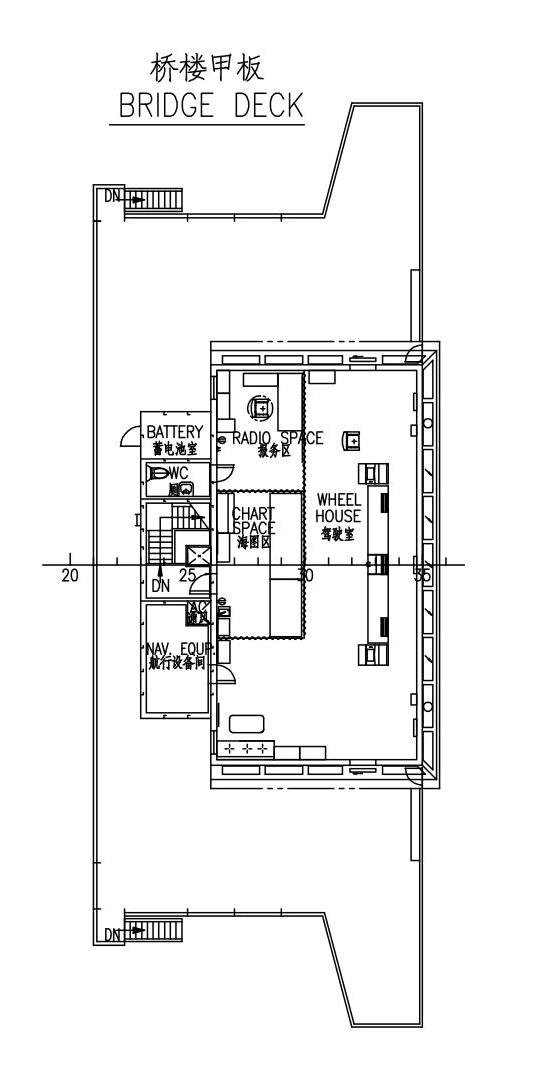
\includegraphics[width=15cm, height=15cm]{bdeck.jpg}};
 
% Create scope with normalized axes
\begin{scope}[
x={($0.1*(image.south east)$)},
y={($0.1*(image.north west)$)}]
 
% Grid
  %  \draw[lightgray,step=1] (image.south west) grid (image.north east);
 
% Labels
 
         \draw[stealth-, very thick,black] (2,4) -- ++(7,2.2)
        node[right,white,fill=black]{\small VCP-2};
        \draw[stealth-, very thick,black] (6,2) -- ++(4,2.2)
        node[right,white,fill=black]{\small VCP-1};
               \draw[stealth-, very thick,black] (6,5) -- ++(4,2.2)
        node[right,white,fill=black]{\small SCP-88};
\end{scope}
 
\end{tikzpicture}
\end{center}


\section{Analysis Results}

The following colour coding is used throughout all parts of this report for
providing a better overview and clarity.

\renewcommand{\arraystretch}{1.4}
\begin{center}
\begin{table}[H]
\begin{tabular}{|ll|l|ll|}
\hline
\multicolumn{2}{|l|}{\textbf{Hazardous Material}}          & \textbf{Abbreviation} & \multicolumn{2}{l|}{\textbf{Colour}}                   \\ \hline
\multicolumn{1}{|l|}{A-1} & Asbestos                       & Asb                   & \multicolumn{1}{l|}{\cellcolor[HTML]{3531FF}} & Blue   \\ \hline
\multicolumn{1}{|l|}{A-2} & Polychlorinated Biphenyl (PCB) & PCB                   & \multicolumn{1}{l|}{\cellcolor[HTML]{6200C9}} & Purple \\ \hline
\multicolumn{1}{|l|}{A-3}    &  Ozone Depleting Substances (ODS)                               &         ODS   &           \multicolumn{1}{l|}{\cellcolor[HTML]{EBF909}} & Yellow      \\ \hline
\multicolumn{1}{|l|}{A-5 }    &  Perfluorooctane Sulfonic Acid (PFOS)                               &         PFOS    &           \multicolumn{1}{l|}{\cellcolor[HTML]{F9BA09}} & Orange      \\ \hline
\multicolumn{1}{|l|}{B-1 }    &  Cadmium (and compounds)                               &         Cd    &           \multicolumn{1}{l|}{\cellcolor[HTML]{900C3F}} & Maroon      \\ \hline
\multicolumn{1}{|l|}{B-2 }    &  Chromium (and compounds)                                &         Cr    &           \multicolumn{1}{l|}{\cellcolor[HTML]{9F4C26}} & Brown      \\ \hline
\multicolumn{1}{|l|}{B-3 }    &  Lead (and compounds)                                &         Pb    &           \multicolumn{1}{l|}{\cellcolor[HTML]{908D8C}} & Grey      \\ \hline
\multicolumn{1}{|l|}{B-4 }    &  Mercury (and compounds)                                &         Hg    &           \multicolumn{1}{l|}{\cellcolor[HTML]{A778E9}} & Lavender      \\ \hline
\multicolumn{1}{|l|}{B-5}    &  Polybrominated Biphenyl (PBB)                                &         PBB    &           \multicolumn{1}{l|}{\cellcolor[HTML]{18B0F5}} & Cyan      \\ \hline
\multicolumn{1}{|l|}{B-6 }    &  Polybrominated Diphenyl Ethers (PBDE)                                 &         PBDE    &           \multicolumn{1}{l|}{\cellcolor[HTML]{F518C7}} & Magenta      \\ \hline
\multicolumn{1}{|l|}{B-7}    &  Polychlorinated Naphthalenes (Cl3) )                                 &         PCN    &           \multicolumn{1}{l|}{\cellcolor[HTML]{DEF518}} & Lime      \\ \hline
\multicolumn{1}{|l|}{B-8 }    &  Radioactive Material                                 &         Radio    &           \multicolumn{1}{l|}{\cellcolor[HTML]{6DF518}} & Green      \\ \hline
\multicolumn{1}{|l|}{B-9}    &  Certain Short Chain Chlorinated Paraffins                                 &         SCCP    &           \multicolumn{1}{l|}{\cellcolor[HTML]{F518D4}} & Pink      \\ \hline
\multicolumn{1}{|l|}{B-10}    &  Hexabromocyclododecane (HBCDD)                                 &         HBCDD    &           \multicolumn{1}{l|}{\cellcolor[HTML]{0B421B}} & Teal      \\ \hline
\end{tabular}
\end{table}
\end{center}

\subsection{Materials containing Asbestos}


\renewcommand{\arraystretch}{1.4}
\begin{center}
\begin{table}[H]
\begin{tabular}{|l|l|l|l|l|}
\hline
\textbf{No} & \textbf{Name} & \textbf{Location}                                                           & \textbf{Object to check}                                                        & \textbf{Remarks}                                                                                                                                       \\ \hline
S-78        & VMS-S077      & \begin{tabular}[c]{@{}l@{}}E/R 2nd deck plan,\\ E/R 2nd deck\end{tabular}   & \begin{tabular}[c]{@{}l@{}}M/E JW preheater,\\ Flange packing\end{tabular}      & Asbestos - Contained 1\% - 15\%, Chrysotile Asbestos Asbestos containing materials needs to be managed and removed following Flag and Class guidelines \\ \hline
S-97        & VMS-S096      & \begin{tabular}[c]{@{}l@{}}Engine Casing\\ Plan, Engine casing\end{tabular} & \begin{tabular}[c]{@{}l@{}}Boiler and\\ economizer, door\\ packing\end{tabular} & Asbestos - Contained 1\% - 15\%, Chrysotile Asbestos Asbestos containing materials needs to be managed and removed following Flag and Class guidelines \\ \hline
\end{tabular}
\end{table}
\end{center}

\subsection{Materials containing Lead (and compounds)}


\renewcommand{\arraystretch}{1.4}
\begin{center}
\begin{table}[H]
\begin{tabular}{|>{\centering\arraybackslash}m{1cm}|>{\centering\arraybackslash}m{1cm}|>{\centering\arraybackslash}m{4cm}|>{\centering\arraybackslash}m{3.6cm}|>{\centering\arraybackslash}m{3.6cm}|}
\hline
\textbf{No} & \textbf{Name} & \textbf{Location}                                                           & \textbf{Object to check}                                                        & \textbf{Remarks}                                                                                                                                       \\ \hline
V-1         &       & \begin{tabular}[c]{@{}l@{}}NAV. BRI. DECK, \\ Battery room\end{tabular}   & \begin{tabular}[c]{@{}l@{}}M/E JW preheater,\\ Flange packing\end{tabular}      & Lead (and compounds) -
Contained
11 kg x 24 = 264 kg, Lead Acid Battery \\ \hline
S-2         & VMS-S002      & \begin{tabular}[c]{@{}l@{}}NAV. BRI. DECK, \\
Open deck ,\\
Superstructure , \\
Crane, Funnel, \\
Wall, body of 
crane \\ , railings\end{tabular} & \begin{tabular}[c]{@{}l@{}}Wall Paint, Coating\\ packing\end{tabular} & Lead (and compounds) -
Contained
2700 mg / Kg, Sigmacover 456 Buff 3142 \\ \hline
\end{tabular}
\end{table}
\end{center}

\section{Summary of Hazardous Materials}

\renewcommand{\arraystretch}{1.4}
\begin{center}
% Please add the following required packages to your document preamble:
% \usepackage{multirow}
\begin{table}[H]
\begin{tabular}{|>{\centering\arraybackslash}m{3.6cm}|>{\centering\arraybackslash}m{2cm}>{\centering\arraybackslash}m{2cm}>{\centering\arraybackslash}m{1.8cm}|>{\centering\arraybackslash}m{3.7cm}>{\centering\arraybackslash}m{3cm}>{\centering\arraybackslash}m{1cm}>{\centering\arraybackslash}m{2cm}|} %{|l|lll|llll|}
\hline
\multirow{2}{*}{\textbf{Hazardous Materials}} & \multicolumn{3}{l|}{\textbf{Check Type}}                                                     & \multicolumn{4}{l|}{\textbf{Check Result}}                                                                                                            \\ \cline{2-8} 
                                              & \multicolumn{1}{l|}{\textbf{Sample}} & \multicolumn{1}{l|}{\textbf{Visual}} & \textbf{Total} & \multicolumn{1}{l|}{\textbf{Contained}} & \multicolumn{1}{l|}{\textbf{PCHM}} & \multicolumn{1}{l|}{\textbf{Below Threshold}} & \textbf{Not Contained} \\ \hline
A-1 Asbestos                                  & \multicolumn{1}{l|}{85}              & \multicolumn{1}{l|}{5}               & 90             & \multicolumn{1}{l|}{2}                  & \multicolumn{1}{l|}{-}             & \multicolumn{1}{l|}{-}                        & 88                     \\ \hline
A-2 Polychlorinated Biphenyl (PCB)            & \multicolumn{1}{l|}{10}              & \multicolumn{1}{l|}{2}               & 12             & \multicolumn{1}{l|}{-}                  & \multicolumn{1}{l|}{-}             & \multicolumn{1}{l|}{-}                        & 12                     \\ \hline
A-3 Ozone Depleting Substances (ODS)          & \multicolumn{1}{l|}{1}               & \multicolumn{1}{l|}{5}               & 6              & \multicolumn{1}{l|}{-}                  & \multicolumn{1}{l|}{-}             & \multicolumn{1}{l|}{-}                        & 6                      \\ \hline
A-4 Organotin Compounds                       & \multicolumn{1}{l|}{-}               & \multicolumn{1}{l|}{-}               & -              & \multicolumn{1}{l|}{-}                  & \multicolumn{1}{l|}{-}             & \multicolumn{1}{l|}{-}                        & -                      \\ \hline
A-5 Perfluorooctane Sulfonic Acid (PFOS)      & \multicolumn{1}{l|}{3}               & \multicolumn{1}{l|}{-}               & 3              & \multicolumn{1}{l|}{-}                  & \multicolumn{1}{l|}{-}             & \multicolumn{1}{l|}{-}                        & -                      \\ \hline
B-1 Cadmium (and compounds)                   & \multicolumn{1}{l|}{5}               & \multicolumn{1}{l|}{-}               & 5              & \multicolumn{1}{l|}{-}                  & \multicolumn{1}{l|}{-}             & \multicolumn{1}{l|}{-}                        & 5                      \\ \hline
B-2 Chromium (and compounds)                  & \multicolumn{1}{l|}{5}               & \multicolumn{1}{l|}{-}               & 5              & \multicolumn{1}{l|}{-}                  & \multicolumn{1}{l|}{-}             & \multicolumn{1}{l|}{-}                        & 5                      \\ \hline
B-3 Lead (and compounds)                      & \multicolumn{1}{l|}{6}               & \multicolumn{1}{l|}{4}               & 10             & \multicolumn{1}{l|}{8}                  & \multicolumn{1}{l|}{-}             & \multicolumn{1}{l|}{1}                        & 1                      \\ \hline
B-4 Mercury (and compounds)                   & \multicolumn{1}{l|}{5}               & \multicolumn{1}{l|}{1}               & 6              & \multicolumn{1}{l|}{-}                  & \multicolumn{1}{l|}{-}             & \multicolumn{1}{l|}{-}                        & 6                      \\ \hline
B-5 Polybrominated Biphenyl (PBB)             & \multicolumn{1}{l|}{1}               & \multicolumn{1}{l|}{-}               & 1              & \multicolumn{1}{l|}{-}                  & \multicolumn{1}{l|}{-}             & \multicolumn{1}{l|}{-}                        & 1                      \\ \hline
B-6 Polybrominated Diphenyl Ethers (PBDE)     & \multicolumn{1}{l|}{1}               & \multicolumn{1}{l|}{-}               & 1              & \multicolumn{1}{l|}{-}                  & \multicolumn{1}{l|}{-}             & \multicolumn{1}{l|}{-}                        & 1                      \\ \hline
B-7 Polychlorinated Naphthalenes              & \multicolumn{1}{l|}{-}               & \multicolumn{1}{l|}{-}               & -              & \multicolumn{1}{l|}{-}                  & \multicolumn{1}{l|}{-}             & \multicolumn{1}{l|}{-}                        & -                      \\ \hline
B-8 Radioactive Material                      & \multicolumn{1}{l|}{-}               & \multicolumn{1}{l|}{2}               & 2              & \multicolumn{1}{l|}{-}                  & \multicolumn{1}{l|}{-}             & \multicolumn{1}{l|}{-}                        & 2                      \\ \hline
B-9 Certain Short Chain Chlorinated Paraffins & \multicolumn{1}{l|}{-}               & \multicolumn{1}{l|}{-}               & -              & \multicolumn{1}{l|}{-}                  & \multicolumn{1}{l|}{-}             & \multicolumn{1}{l|}{-}                        & -                      \\ \hline
B-10 Hexabromocyclododecane (HBCDD)           & \multicolumn{1}{l|}{4}               & \multicolumn{1}{l|}{-}               & 4              & \multicolumn{1}{l|}{-}                  & \multicolumn{1}{l|}{-}             & \multicolumn{1}{l|}{-}                        & 4                      \\ \hline
\textbf{Total}                                & \multicolumn{1}{l|}{\textbf{126}}    & \multicolumn{1}{l|}{\textbf{19}}     & \textbf{145}   & \multicolumn{1}{l|}{\textbf{10}}        & \multicolumn{1}{l|}{\textbf{0}}    & \multicolumn{1}{l|}{\textbf{1}}               & \textbf{134}           \\ \hline
\end{tabular}
\end{table}
\end{center}


\section{Documentation of check points}

The following colour code is used for marking of check points. Different shapes
are used to distinguish between sampling checks and visual checks.

\renewcommand{\arraystretch}{1.4}
\begin{center}
% Please add the following required packages to your document preamble:
% \usepackage{multirow}
\begin{table}[H]
\begin{tabular}{|ll|ll|ll|ll|}
\hline
\multicolumn{2}{|l|}{\multirow{2}{*}{\textbf{Hazardous Material}}}                                                        & \multicolumn{2}{l|}{\textbf{Not Contained}}            & \multicolumn{2}{l|}{\textbf{Below Threshold}}          & \multicolumn{2}{l|}{\textbf{Contained or PCHM}}        \\ \cline{3-8} 
\multicolumn{2}{|l|}{}                                                                                                    & \multicolumn{1}{l|}{\textit{Sample}} & \textit{Visual} & \multicolumn{1}{l|}{\textit{Sample}} & \textit{Visual} & \multicolumn{1}{l|}{\textit{Sample}} & \textit{Visual} \\ \hline
\multicolumn{1}{|l|}{A-1}           & Asbestos                                                                            & \multicolumn{1}{l|}{}                &                 & \multicolumn{1}{l|}{}                &                 & \multicolumn{1}{l|}{}                &                 \\ \hline
\multicolumn{1}{|l|}{A-2}           & Polychlorinated Biphenyl (PCB)                                                      & \multicolumn{1}{l|}{}                &                 & \multicolumn{1}{l|}{}                &                 & \multicolumn{1}{l|}{}                &                 \\ \hline
\multicolumn{1}{|l|}{A-3}           & Ozone Depleting Substances (ODS)                                                    & \multicolumn{1}{l|}{}                &                 & \multicolumn{1}{l|}{}                &                 & \multicolumn{1}{l|}{}                &                 \\ \hline
\multicolumn{1}{|l|}{A-5}           & Perfluorooctane Sulfonic Acid (PFOS)                                                & \multicolumn{1}{l|}{}                &                 & \multicolumn{1}{l|}{}                &                 & \multicolumn{1}{l|}{}                &                 \\ \hline
\multicolumn{1}{|l|}{B-1}           & Cadmium (and compounds)                                                             & \multicolumn{1}{l|}{}                &                 & \multicolumn{1}{l|}{}                &                 & \multicolumn{1}{l|}{}                &                 \\ \hline
\multicolumn{1}{|l|}{B-2}           & Chromium (and compounds)                                                            & \multicolumn{1}{l|}{}                &                 & \multicolumn{1}{l|}{}                &                 & \multicolumn{1}{l|}{}                &                 \\ \hline
\multicolumn{1}{|l|}{B-3}           & Lead (and compounds)                                                                & \multicolumn{1}{l|}{}                &                 & \multicolumn{1}{l|}{}                &                 & \multicolumn{1}{l|}{}                &                 \\ \hline
\multicolumn{1}{|l|}{B-4}           & Mercury (and compounds)                                                             & \multicolumn{1}{l|}{}                &                 & \multicolumn{1}{l|}{}                &                 & \multicolumn{1}{l|}{}                &                 \\ \hline
\multicolumn{1}{|l|}{B-5}           & Polybrominated Biphenyl (PBB)                                                       & \multicolumn{1}{l|}{}                &                 & \multicolumn{1}{l|}{}                &                 & \multicolumn{1}{l|}{}                &                 \\ \hline
\multicolumn{1}{|l|}{B-6}           & Polybrominated Diphenyl Ethers (PBDE)                                               & \multicolumn{1}{l|}{}                &                 & \multicolumn{1}{l|}{}                &                 & \multicolumn{1}{l|}{}                &                 \\ \hline
\multicolumn{1}{|l|}{B-7}           & Polychlorinated Naphthalenes                                                        & \multicolumn{1}{l|}{}                &                 & \multicolumn{1}{l|}{}                &                 & \multicolumn{1}{l|}{}                &                 \\ \hline
\multicolumn{1}{|l|}{B-8}           & Radioactive Material                                                                & \multicolumn{1}{l|}{}                &                 & \multicolumn{1}{l|}{}                &                 & \multicolumn{1}{l|}{}                &                 \\ \hline
\multicolumn{1}{|l|}{B-9}           & \begin{tabular}[c]{@{}l@{}}Certain Short Chain Chlorinated\\ Paraffins\end{tabular} & \multicolumn{1}{l|}{}                &                 & \multicolumn{1}{l|}{}                &                 & \multicolumn{1}{l|}{}                &                 \\ \hline
\multicolumn{1}{|l|}{B-10} & Hexabromocyclododecane (HBCDD)                                                      & \multicolumn{1}{l|}{}                &                 & \multicolumn{1}{l|}{}                &                 & \multicolumn{1}{l|}{}                &                 \\ \hline
\end{tabular}
\end{table}
\end{center}

\subsection{Check points on Deck: NAV. BRI. DECK}

\begin{center}
    

\begin{tikzpicture}
 
% Include the image in a node
\node [
    above right,
    inner sep=0] (image) at (0,0) {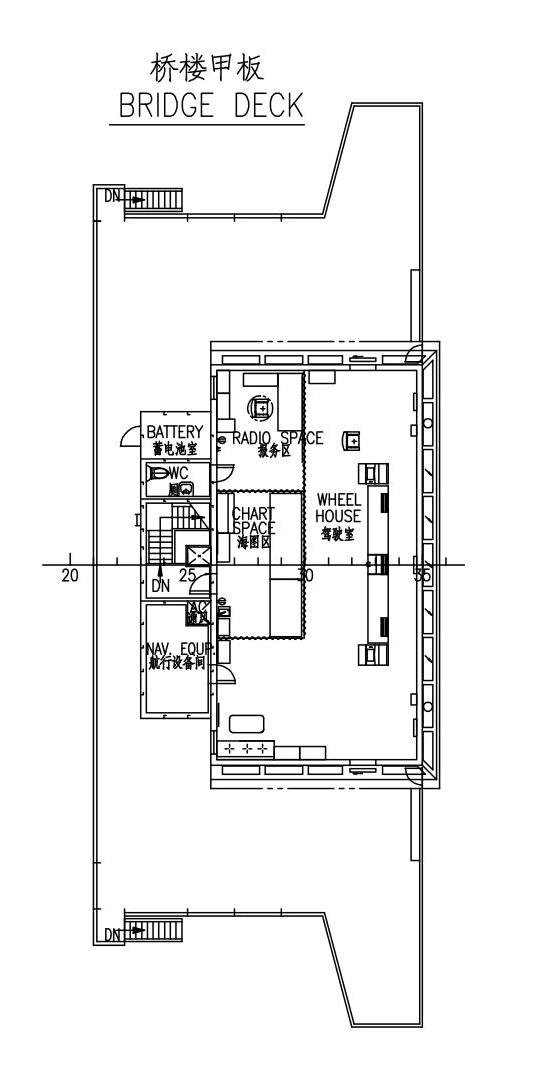
\includegraphics[width=15cm, height=15cm]{bdeck.jpg}};
 
% Create scope with normalized axes
\begin{scope}[
x={($0.1*(image.south east)$)},
y={($0.1*(image.north west)$)}]
 
% Grid
  %  \draw[lightgray,step=1] (image.south west) grid (image.north east);
 
% Labels
 
         \draw[stealth-, very thick,black] (2,4) -- ++(7,2.2)
        node[right,white,fill=black]{\small VCP-2};
        \draw[stealth-, very thick,black] (6,2) -- ++(4,2.2)
        node[right,white,fill=black]{\small VCP-1};
               \draw[stealth-, very thick,black] (6,5) -- ++(4,2.2)
        node[right,white,fill=black]{\small SCP-88};
\end{scope}
 
\end{tikzpicture}
\end{center}


\section{Photos of Samples and Visual Checks}

\subsection{Photos of Samples}

\subsection{Photos of Visuals}

\section{Attachments}

This section contains all the PDF Attachments.

\subsection{Lab Result}
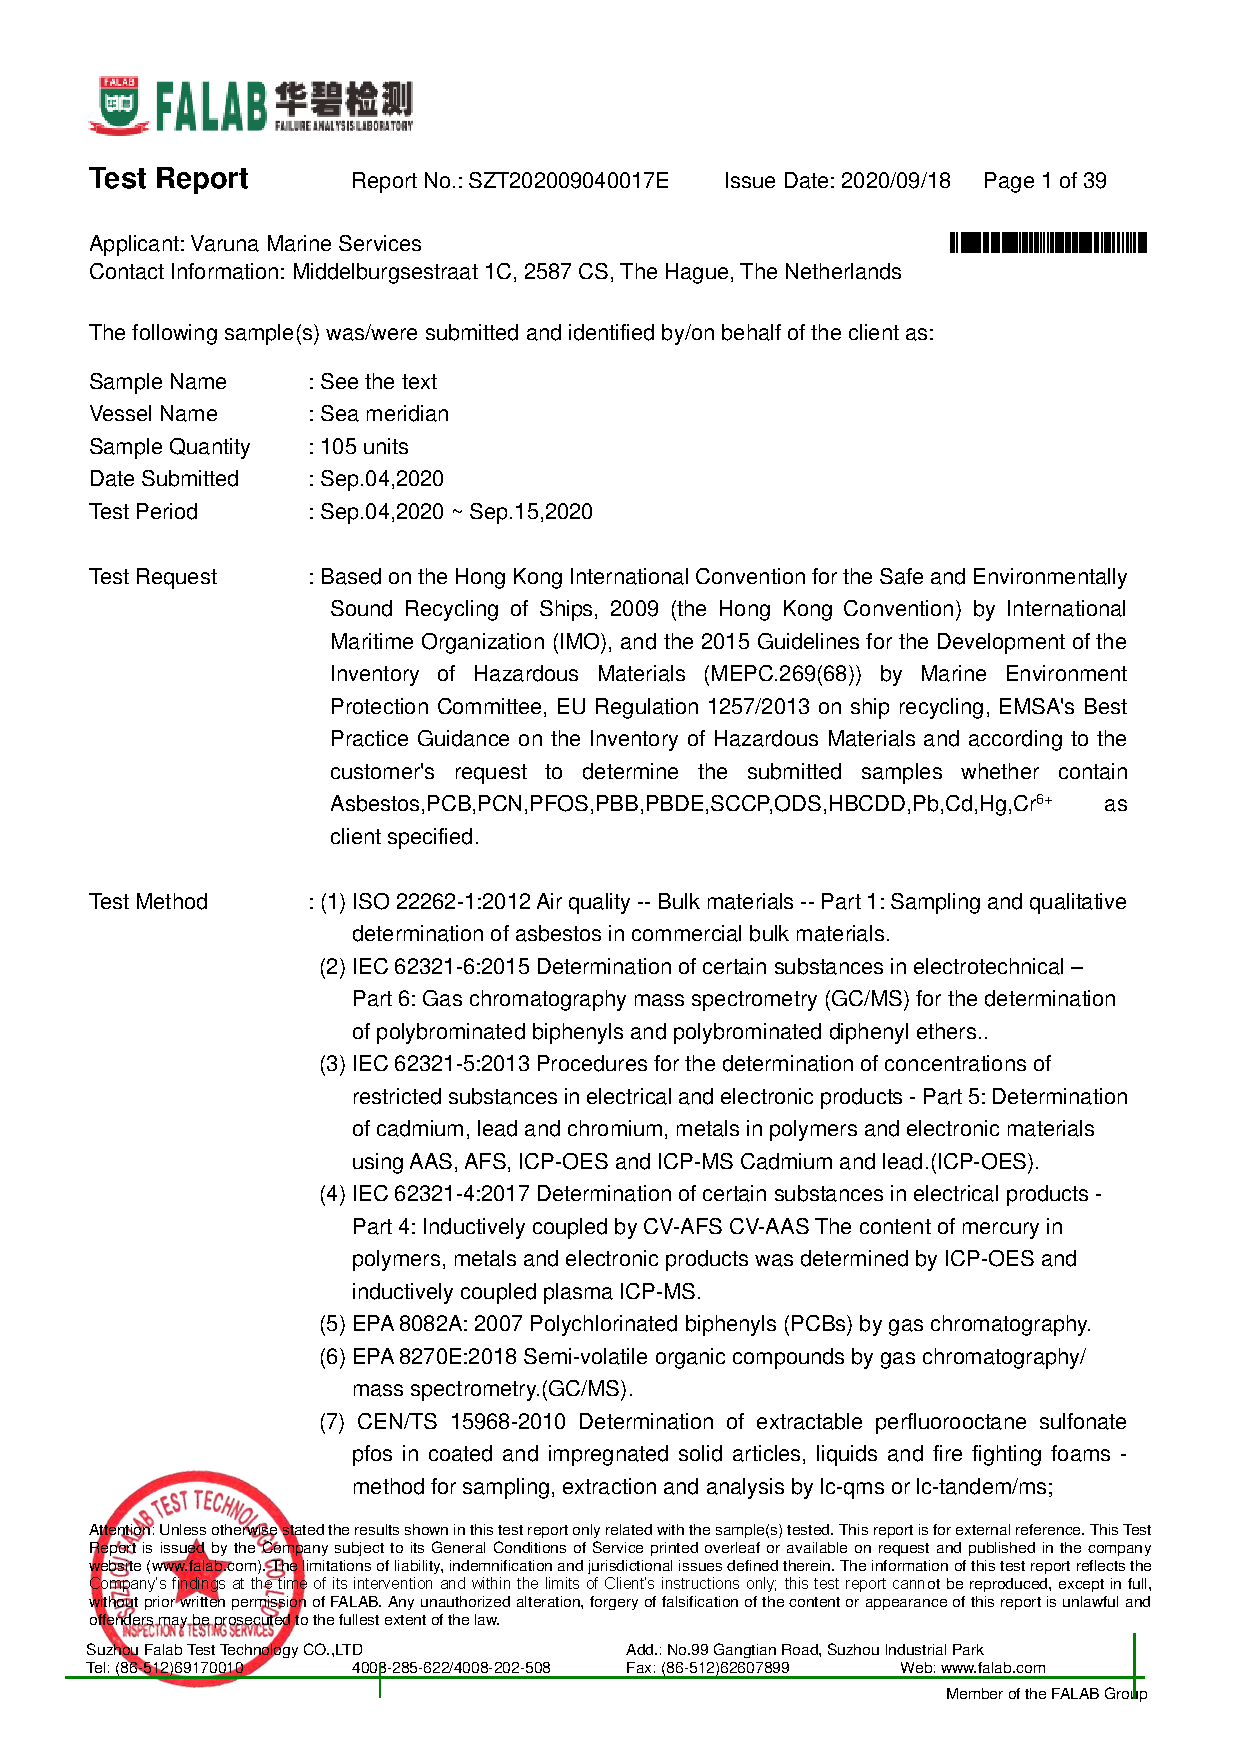
\includepdf[pages=-]{assets/Lab_result.pdf}
\subsection{Hazmat Certificate}

\includepdf[pages=-]{assets/Hazmat_cert.pdf}


% ------------------------------------------
% BIBLIOGRAPHY
% ------------------------------------------
\newpage
% \bibliography{references}

% ------------------------------------------
% APPENDICES & ATTACHMENTS
% ------------------------------------------
\newpage

\renewcommand{\thesubsection}{\Alph{subsection}}



\end{document}